\documentclass[UTF8,zihao=-4]{ctexart}
\usepackage[a4paper,margin=2.5cm]{geometry}
\usepackage{amsmath, amssymb, amsthm}
\usepackage{bm}
\usepackage{hyperref}
\usepackage{graphicx}
\usepackage{caption}
\usepackage{listings}
\usepackage{xcolor}
\usepackage{float}
\usepackage{placeins}
\graphicspath{{figures/}}

% Code style
\lstdefinestyle{code}{
  basicstyle=\ttfamily\small,
  numbers=left,
  numberstyle=\tiny,
  numbersep=8pt,
  keywordstyle=\color{blue},
  commentstyle=\color{teal!70!black},
  stringstyle=\color{orange!70!black},
  showstringspaces=false,
  breaklines=true,
  frame=single,
  framerule=0.3pt,
  rulecolor=\color{black!15}
}
\lstset{style=code}

\title{优化与正则化技巧实战}
\author{}
\date{\today}

\begin{document}
\maketitle
\tableofcontents
\FloatBarrier

\section{自适应优化器:Adam、RMSprop 及其家族}
自适应优化器通过为每个参数维护独立的统计量来自适应地调整学习率,使得模型能够在病态曲面或噪声目标函数上更快收敛。常见方法都会累计梯度的一阶与二阶矩信息。

\subsection{RMSprop}
RMSprop 维护梯度平方的指数滑动平均:
\begin{align}
  \mathbf{v}_t &= \rho \mathbf{v}_{t-1} + (1-\rho)\,\nabla_{\boldsymbol{\theta}} \mathcal{L}_t \odot \nabla_{\boldsymbol{\theta}} \mathcal{L}_t, \\
  \boldsymbol{\theta}_{t+1} &= \boldsymbol{\theta}_t - \eta \frac{\nabla_{\boldsymbol{\theta}} \mathcal{L}_t}{\sqrt{\mathbf{v}_t + \epsilon}},
\end{align}
其中 $\rho \approx 0.9$,$\epsilon \approx 10^{-8}$ 防止除零。平方和的累积抑制了在陡峭方向上的步长,有效缓解了学习率选择问题。

\subsection{Adam 与 AdamW}
Adam 在 RMSprop 的基础上引入动量,计算梯度的一阶与二阶矩:
\begin{align}
  \mathbf{m}_t &= \beta_1 \mathbf{m}_{t-1} + (1-\beta_1)\,\nabla_{\boldsymbol{\theta}} \mathcal{L}_t, \\
  \mathbf{v}_t &= \beta_2 \mathbf{v}_{t-1} + (1-\beta_2)\,\nabla_{\boldsymbol{\theta}} \mathcal{L}_t \odot \nabla_{\boldsymbol{\theta}} \mathcal{L}_t.
\end{align}
偏置校正项消除了初始为零的影响:
\begin{align}
  \hat{\mathbf{m}}_t &= \frac{\mathbf{m}_t}{1-\beta_1^{t}}, &
  \hat{\mathbf{v}}_t &= \frac{\mathbf{v}_t}{1-\beta_2^{t}}.
\end{align}
参数更新因此写为
\begin{equation}
  \boldsymbol{\theta}_{t+1} = \boldsymbol{\theta}_t - \eta \frac{\hat{\mathbf{m}}_t}{\sqrt{\hat{\mathbf{v}}_t} + \epsilon}.
\end{equation}
AdamW 将权重衰减与自适应梯度解耦:
\begin{equation}
  \boldsymbol{\theta}_{t+1} = (1-\eta \lambda)\boldsymbol{\theta}_t - \eta \frac{\hat{\mathbf{m}}_t}{\sqrt{\hat{\mathbf{v}}_t} + \epsilon},
\end{equation}
其中 $\lambda$ 为权重衰减系数,能够更稳定地控制参数范数并提升泛化。

\subsection{更多改进优化器}
\begin{itemize}
  \item \textbf{AdaBelief} 使用梯度与一阶矩之间的偏差来估计方差,在平稳区域具有更小的噪声。
  \item \textbf{AdaFactor} 将二阶矩分解为行、列向量,大幅降低大型模型(如 Transformer)的显存消耗。
  \item \textbf{Yogi} 通过受控的加减更新避免二阶矩无限增大,在稀疏梯度场中更稳定。
\end{itemize}

\begin{figure}[H]
  \centering
  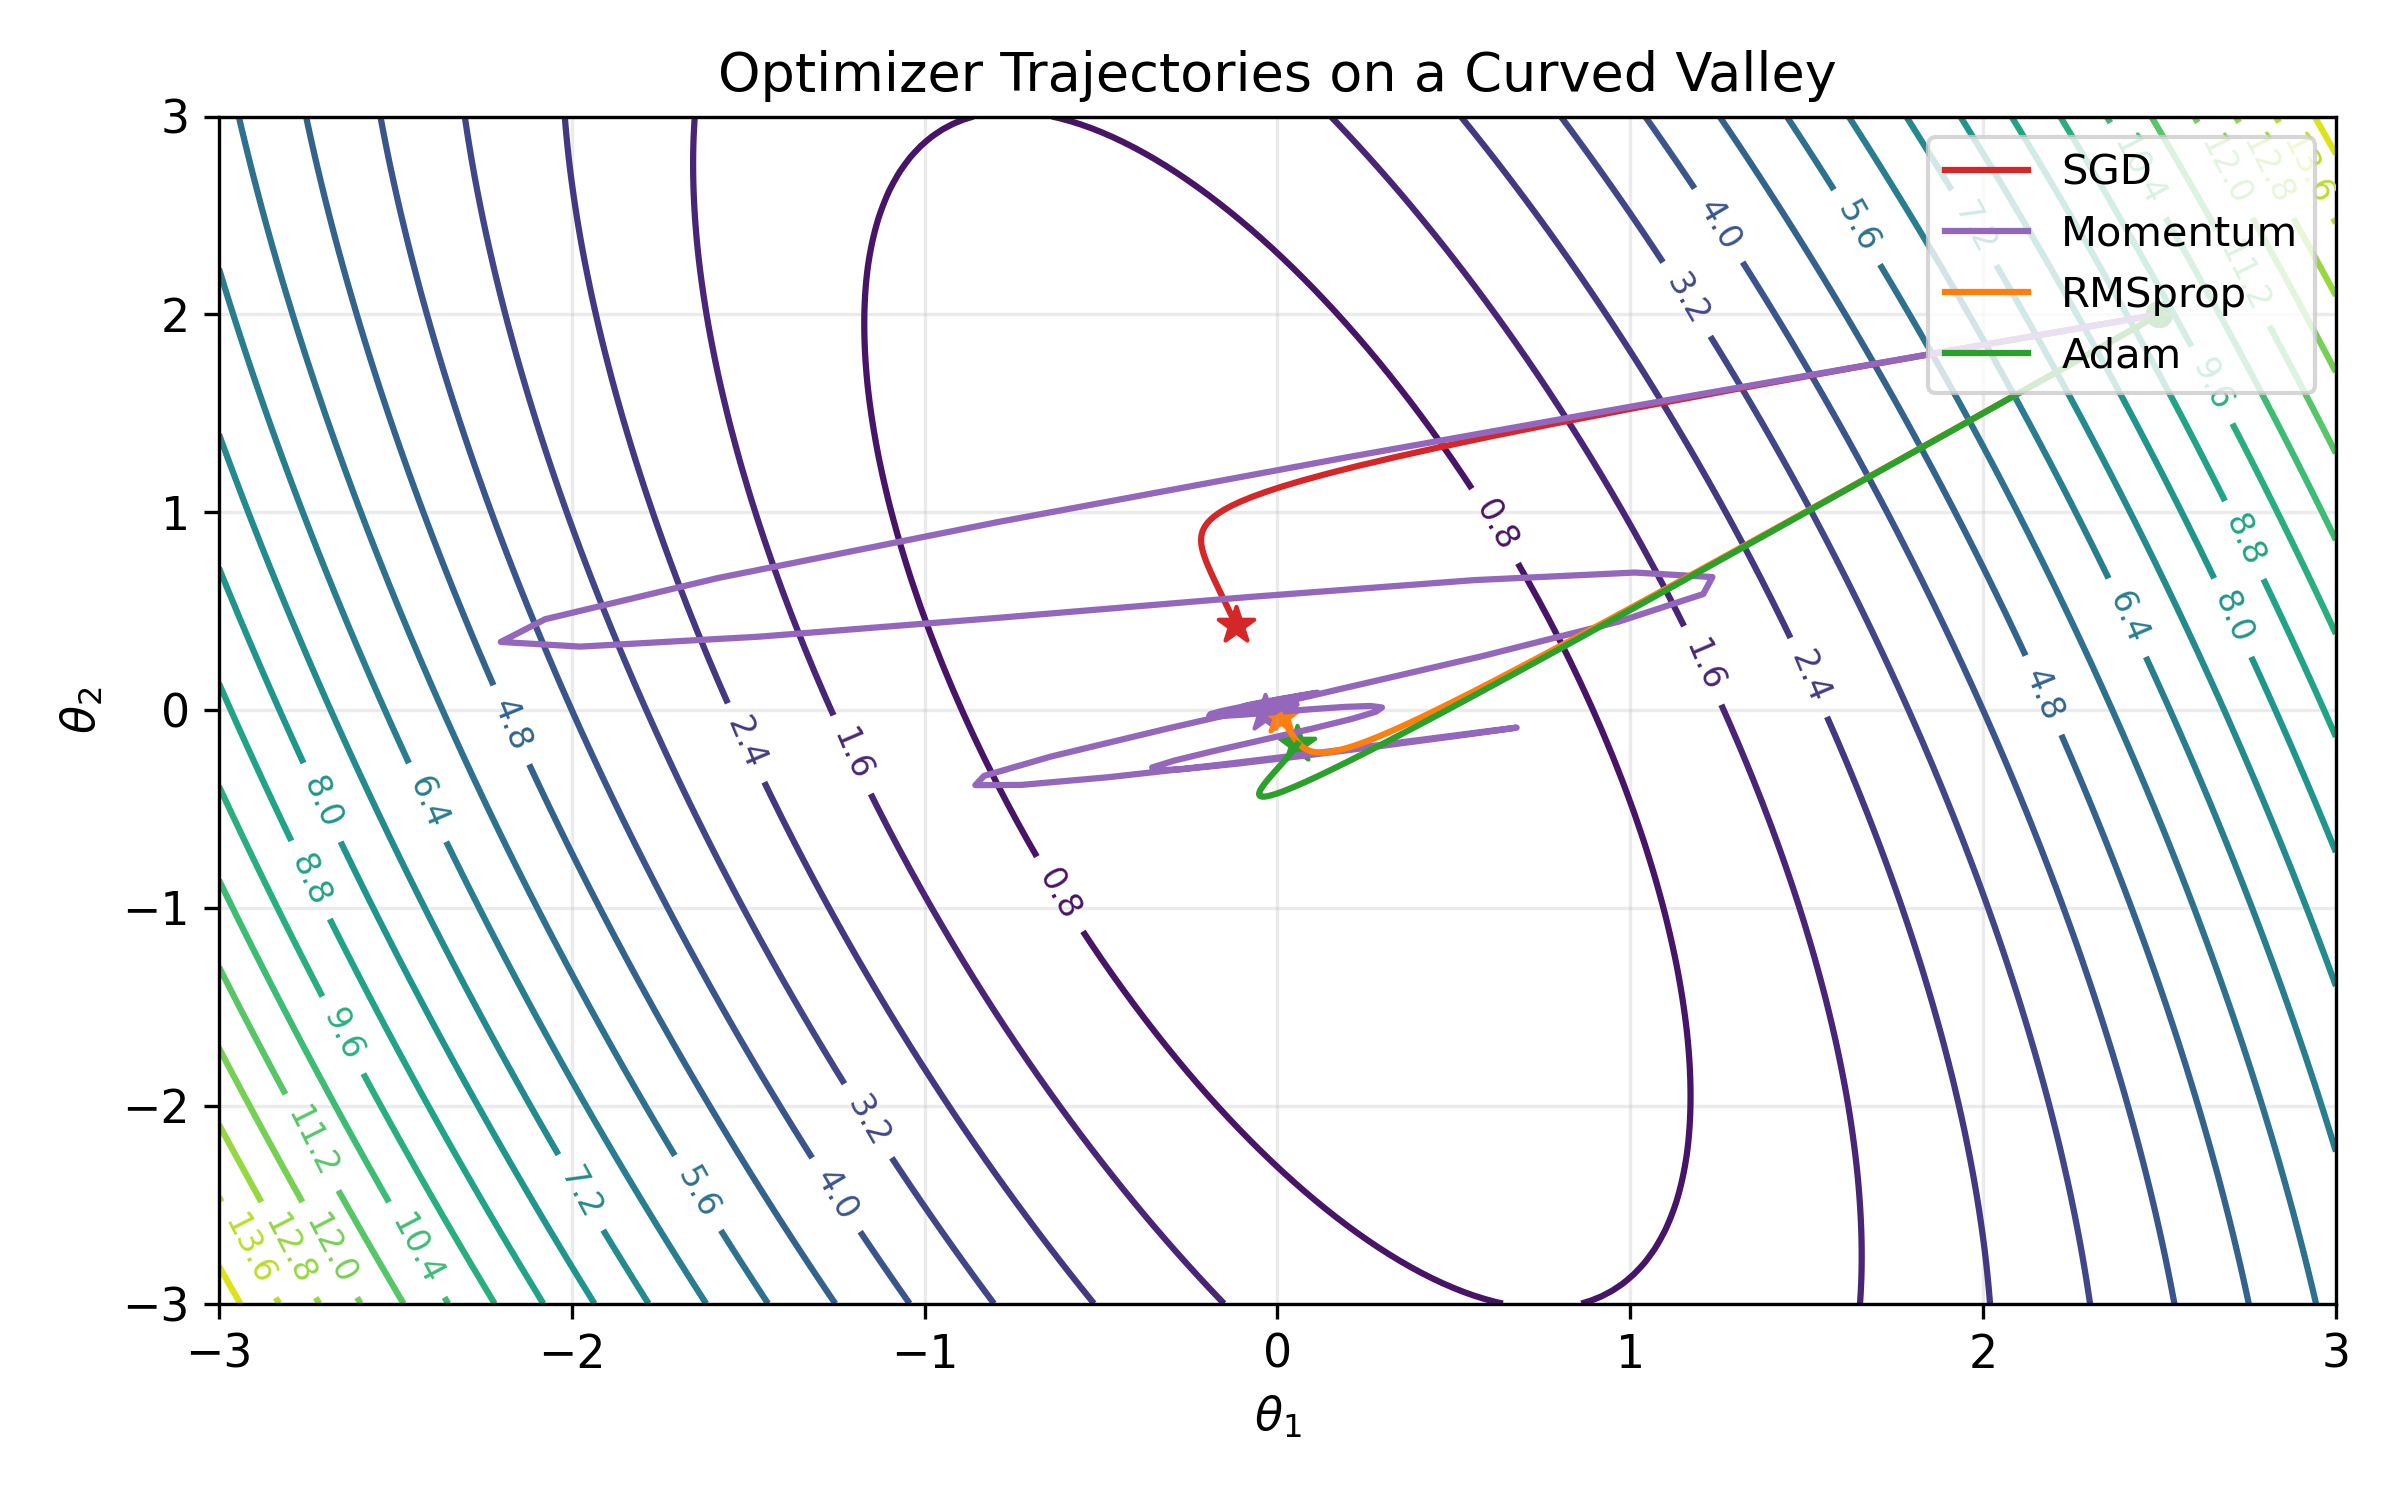
\includegraphics[width=0.8\textwidth]{optimizer_dynamics.png}
  \caption{SGD、动量、RMSprop 与 Adam 在狭长谷底上的优化轨迹对比。自适应方法能够自适应缩放方向梯度。}
  \label{fig:optimizer_dynamics_cn}
\end{figure}
\FloatBarrier

\subsection{实现要点}
大规模训练常组合梯度裁剪、混合精度以及解耦权重衰减。如下 PyTorch 代码展示了带有梯度裁剪和余弦退火的 AdamW:

\begin{lstlisting}[language=Python, caption={结合梯度裁剪与余弦调度的 AdamW 训练循环。}]
import torch
from torch.nn.utils import clip_grad_norm_
from torch.optim.lr_scheduler import CosineAnnealingLR

optimizer = torch.optim.AdamW(model.parameters(), lr=3e-4,
                              betas=(0.9, 0.999), eps=1e-8, weight_decay=0.01)
scheduler = CosineAnnealingLR(optimizer, T_max=1000, eta_min=1e-5)

for step, batch in enumerate(dataloader, start=1):
    loss = compute_loss(model, batch)
    loss.backward()
    clip_grad_norm_(model.parameters(), max_norm=1.0)
    optimizer.step()
    scheduler.step()
    optimizer.zero_grad()
\end{lstlisting}

\section{Batch Normalization 与 Layer Normalization}
归一化层通过稳定激活分布的均值与方差减少层间协变量偏移,显著提升收敛速度并带来一定的正则化效果。

\subsection{Batch Normalization}
对于一个 mini-batch $\mathcal{B} = \{\mathbf{h}_i\}_{i=1}^{m}$,BatchNorm 在特征维度上标准化:
\begin{align}
  \boldsymbol{\mu}_\mathcal{B} &= \frac{1}{m} \sum_{i=1}^{m} \mathbf{h}_i, &
  \boldsymbol{\sigma}_\mathcal{B}^2 &= \frac{1}{m} \sum_{i=1}^{m} (\mathbf{h}_i - \boldsymbol{\mu}_\mathcal{B})^{\odot 2}, \\
  \hat{\mathbf{h}}_i &= \frac{\mathbf{h}_i - \boldsymbol{\mu}_\mathcal{B}}{\sqrt{\boldsymbol{\sigma}_\mathcal{B}^2 + \epsilon}}, &
  \mathbf{y}_i &= \boldsymbol{\gamma} \odot \hat{\mathbf{h}}_i + \boldsymbol{\beta}.
\end{align}
训练阶段使用批统计量,推理阶段则使用滑动平均。由于 BN 会引入批噪声,它在卷积网络中具有良好的正则化效果,但在小批量或序列任务中需要特别处理。

\subsection{Layer Normalization}
LayerNorm 在单个样本的特征维度上归一化:
\begin{equation}
  \mu = \frac{1}{d} \sum_{j=1}^{d} h_j, \quad \sigma^2 = \frac{1}{d} \sum_{j=1}^{d} (h_j - \mu)^2, \quad \hat{h}_j = \frac{h_j - \mu}{\sqrt{\sigma^2 + \epsilon}}.
\end{equation}
随后通过可学习参数 $(\gamma, \beta)$ 恢复尺度与偏移。LN 不依赖 batch 规模,在 Transformer、语言模型等场景中表现稳定。

\subsection{差异与组合实践}
\begin{itemize}
  \item \textbf{对批大小敏感度:} BN 对 batch 规模敏感;LN 对任意 batch 均适用。
  \item \textbf{正则化强度:} BN 的噪声具备隐式正则化;LN 需搭配显式正则化(如 dropout)。
  \item \textbf{跨设备同步:} 分布式训练中 BN 需同步统计量,LN 则无需通信开销。
\end{itemize}

\begin{figure}[H]
  \centering
  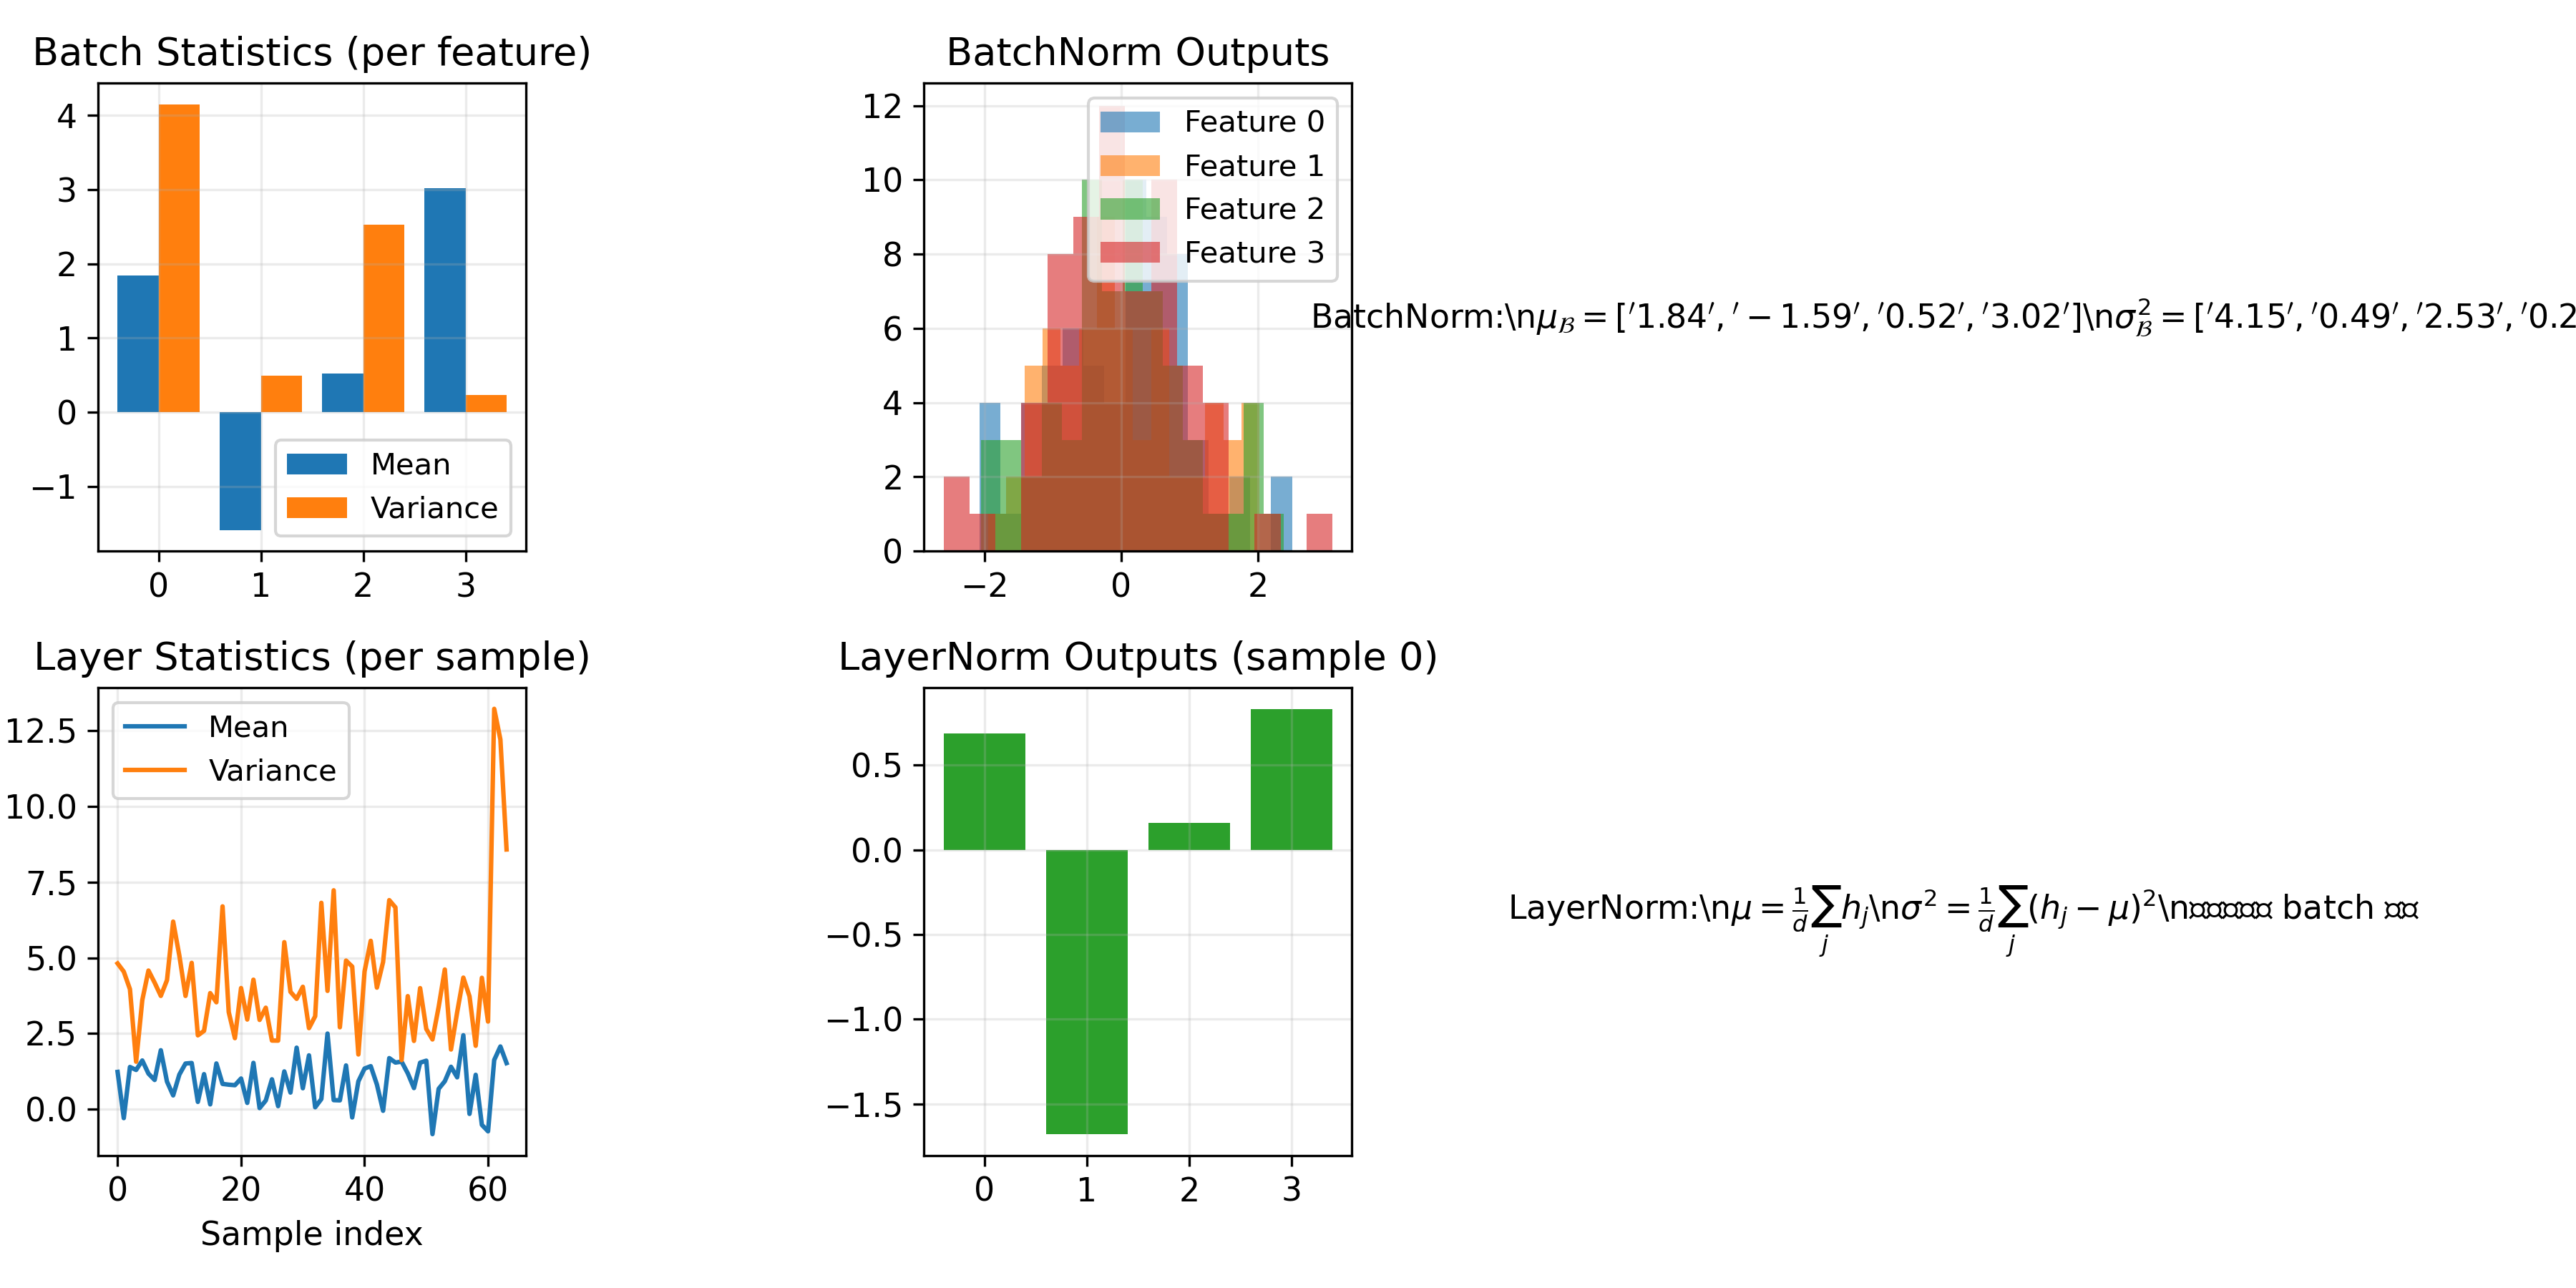
\includegraphics[width=0.8\textwidth]{normalization_comparison.png}
  \caption{BatchNorm 与 LayerNorm 归一化前后特征分布的对比。LN 在每个样本内部进行标准化。}
  \label{fig:normalization_comparison_cn}
\end{figure}
\FloatBarrier

\section{学习率调度与 Warm-up}
合理的学习率策略能够在训练早期快速下降、后期稳定收敛。Warm-up 则避免自适应优化器在统计量尚未稳定时产生过大的步长。

\subsection{阶梯、指数与多项式衰减}
阶梯衰减每隔 $k$ 个 epoch 将学习率乘以 $\gamma < 1$:
\begin{equation}
  \eta_t = \eta_0 \gamma^{\left\lfloor \frac{t}{k} \right\rfloor}.
\end{equation}
指数衰减连续地减小学习率:
\begin{equation}
  \eta_t = \eta_0 \exp(-\lambda t).
\end{equation}
多项式衰减在 $T$ 步内平滑地从 $\eta_0$ 过渡到 $\eta_{\mathrm{end}}$:
\begin{equation}
  \eta_t = \eta_{\mathrm{end}} + (\eta_0 - \eta_{\mathrm{end}})\left(1 - \frac{t}{T}\right)^{p}.
\end{equation}

\subsection{余弦退火与循环策略}
余弦退火将学习率平滑衰减到 $\eta_{\min}$:
\begin{equation}
  \eta_t = \eta_{\min} + \frac{1}{2}(\eta_0 - \eta_{\min})\left(1 + \cos\frac{\pi t}{T}\right).
\end{equation}
循环学习率(CLR)在一个周期内在上下界之间往返,有助于跳出局部极小值。例如三角策略通过线性上升至 $\eta_{\max}$ 再下降到 $\eta_{\min}$。

\subsection{Warm-up}
Warm-up 将学习率在起始 $T_w$ 步内线性升高:
\begin{equation}
  \eta_t =
  \begin{cases}
    \eta_{\mathrm{target}} \frac{t}{T_w}, & 0 \le t \le T_w, \\
    \text{Schedule}(t - T_w), & t > T_w.
  \end{cases}
\end{equation}
Transformer 常采用线性 Warm-up 后接 $\eta_t \propto t^{-1/2}$ 的逆平方衰减。该策略能避免一阶与二阶动量尚未稳定时出现梯度爆炸。

\begin{figure}[H]
  \centering
  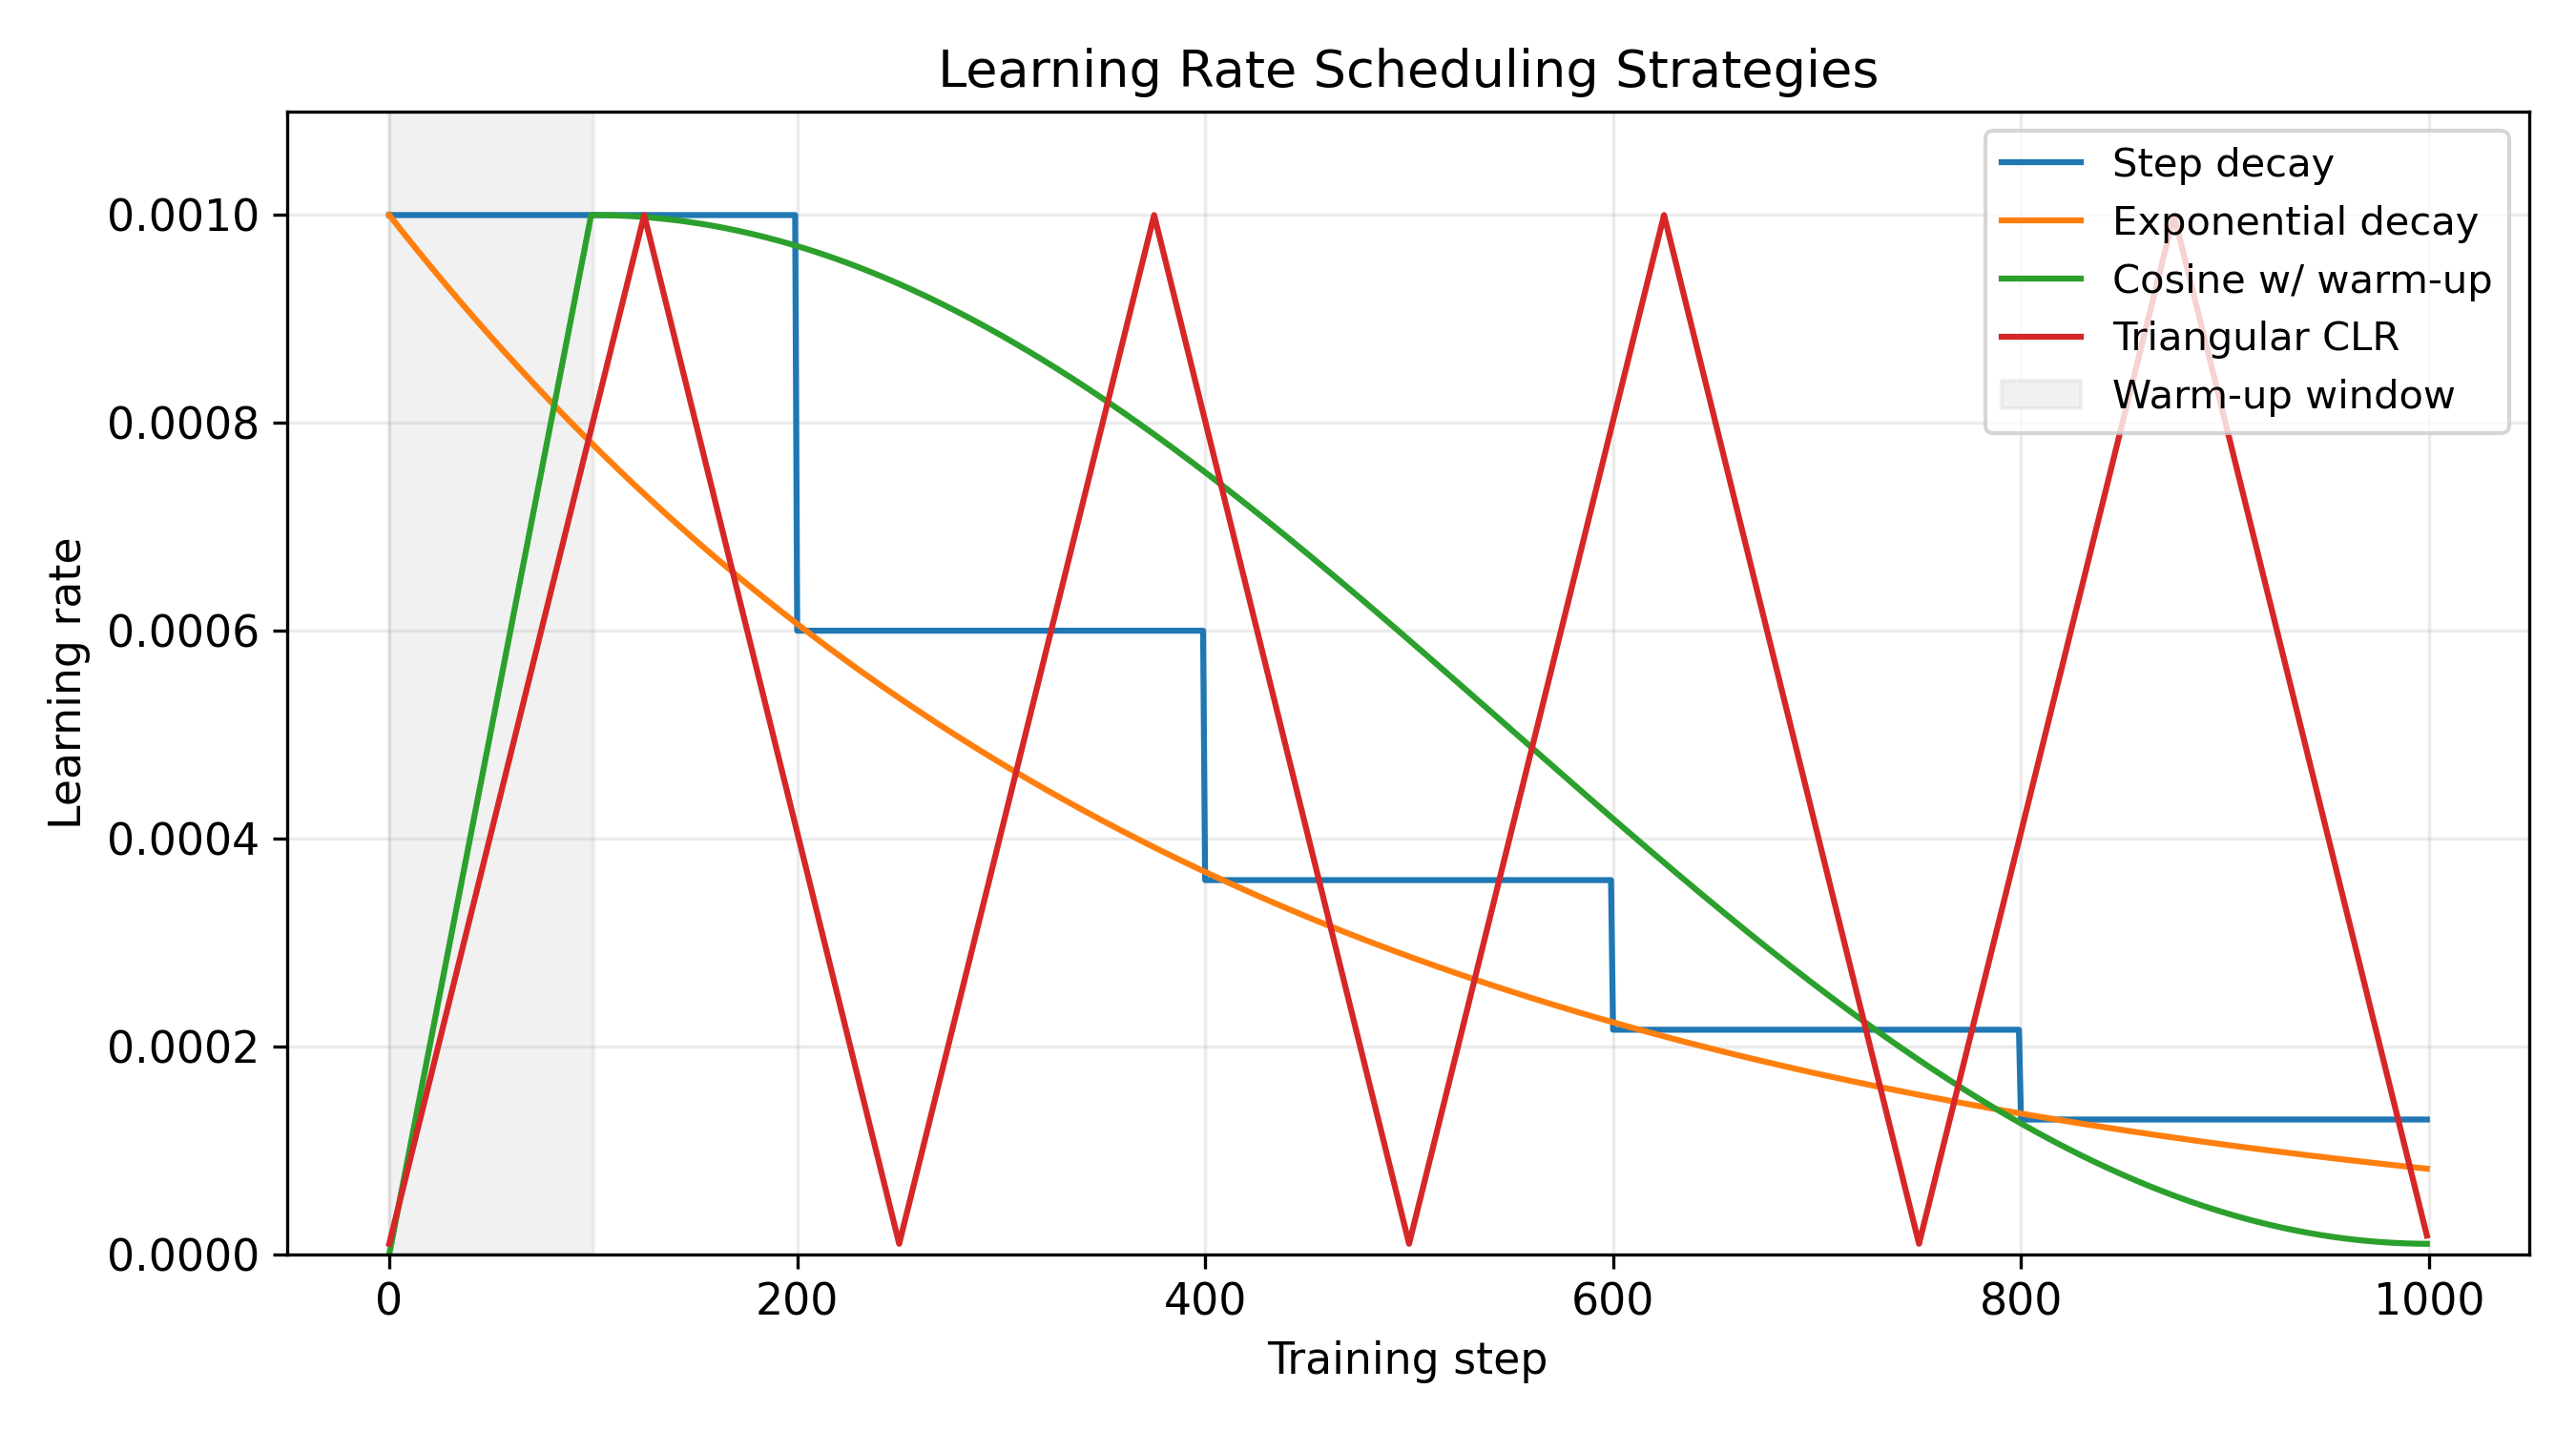
\includegraphics[width=0.85\textwidth]{learning_rate_policies.png}
  \caption{阶梯、余弦、循环与 Warm-up 组合学习率策略示意。}
  \label{fig:learning_rate_policies_cn}
\end{figure}
\FloatBarrier

\section{数据增强与迁移学习}
数据增强扩展了有效训练分布,迁移学习则复用预训练特征,在小样本场景中显著提升性能。

\subsection{经典与高级增强方法}
\begin{itemize}
  \item \textbf{几何增强:} 随机裁剪、翻转、旋转、形变等。
  \item \textbf{光照增强:} 颜色抖动、伽马校正、Cutout、随机遮挡。
  \item \textbf{混合增强:} Mixup 构造 $\tilde{\mathbf{x}} = \lambda \mathbf{x}_i + (1-\lambda)\mathbf{x}_j$、$\tilde{\mathbf{y}} = \lambda \mathbf{y}_i + (1-\lambda)\mathbf{y}_j$。
  \item \textbf{分布扰动:} RandAugment 随机挑选若干操作级联,AugMix 则将多条增强路径加权融合并引入一致性正则。
\end{itemize}

\subsection{迁移学习流程}
迁移学习从来源数据集 $\mathcal{D}_{\mathrm{src}}$ 的预训练权重 $\boldsymbol{\theta}_{\mathrm{pre}}$ 出发,在目标数据集 $\mathcal{D}_{\mathrm{tgt}}$ 上微调:
\begin{align}
  \boldsymbol{\theta}_0 &= \boldsymbol{\theta}_{\mathrm{pre}}, \\
  \boldsymbol{\theta}_{t+1} &= \boldsymbol{\theta}_t - \eta_t \nabla_{\boldsymbol{\theta}} \bigl[\mathcal{L}_{\mathrm{tgt}}(\boldsymbol{\theta}_t) + \lambda \mathcal{R}(\boldsymbol{\theta}_t - \boldsymbol{\theta}_{\mathrm{pre}})\bigr],
\end{align}
其中 $\mathcal{R}$ 可设计为 L2-SP、Fisher 正则等,以限制过度偏离预训练表示。层级自适应学习率(LARS、LAMB)则常用于大模型微调。

\subsection{自监督预训练}
对比学习与掩码预测任务提供了无监督的可迁移特征。SimCLR 的 NT-Xent 损失定义为
\begin{equation}
  \mathcal{L}_{\mathrm{NT-Xent}} = -\sum_{i} \log \frac{\exp(\mathbf{z}_i \cdot \mathbf{z}_{i}' / \tau)}{\sum_{j} \mathbf{1}_{[j \neq i]} \exp(\mathbf{z}_i \cdot \mathbf{z}_j / \tau)},
\end{equation}
通过最大化不同增强视角的相似度来学习表征。后续只需少量标注即可完成下游微调。

\subsection{综合流程示意}
图~\ref{fig:augmentation_transfer_pipeline_cn} 总结了一条常见的管线:数据增强生成多样样本,特征骨干网络进行预训练,再通过任务头进行微调或蒸馏。

\begin{figure}[H]
  \centering
  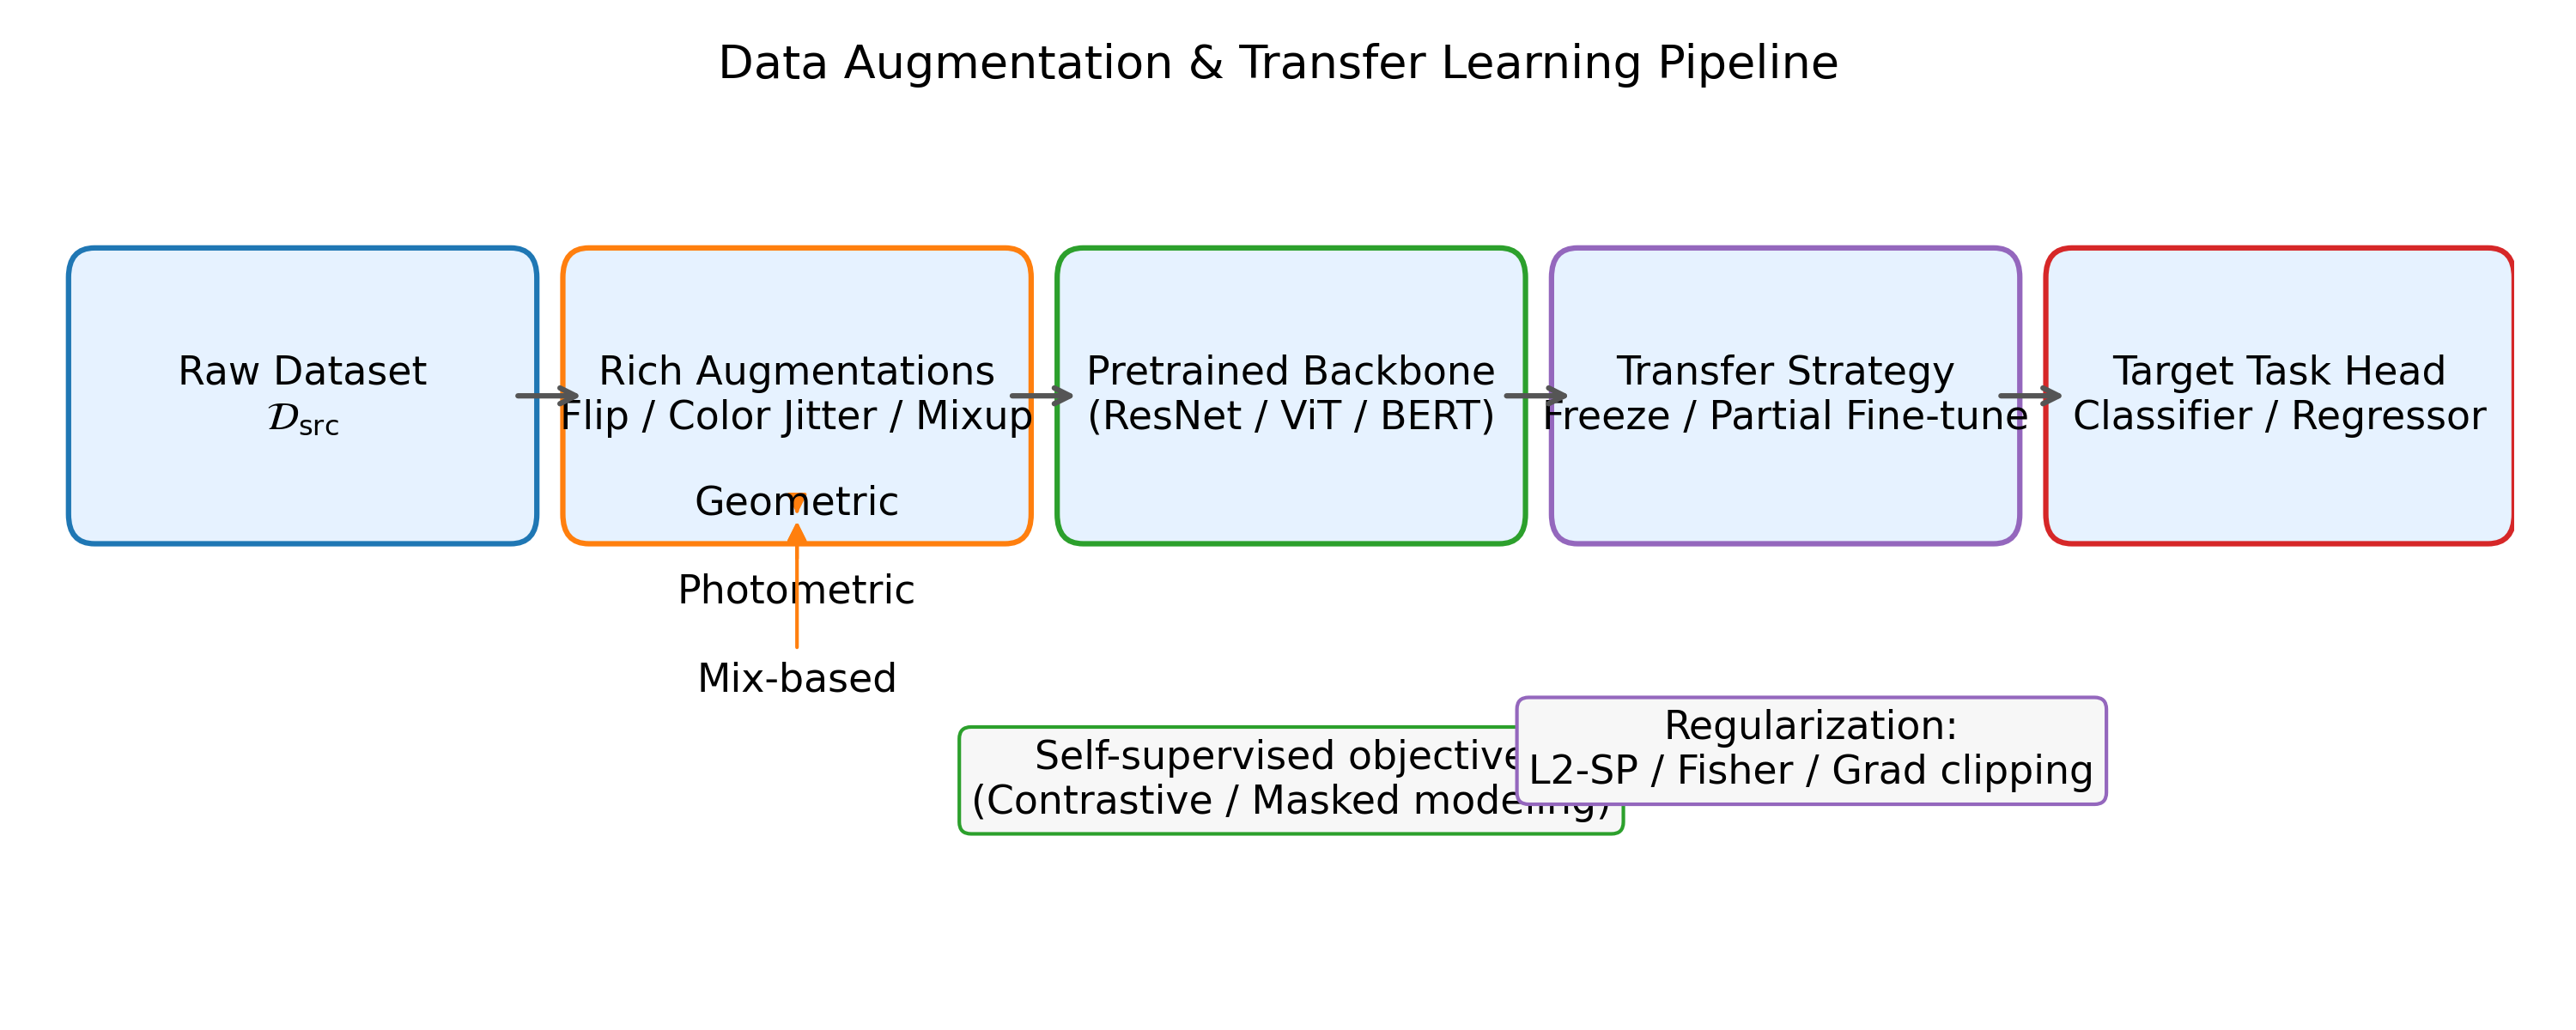
\includegraphics[width=0.9\textwidth]{augmentation_transfer_pipeline.png}
  \caption{数据增强与迁移学习协同的工作流。可选择冻结主干或进行分层微调。}
  \label{fig:augmentation_transfer_pipeline_cn}
\end{figure}
\FloatBarrier

\section*{延伸阅读}
\begin{itemize}
  \item Ilya Loshchilov \& Frank Hutter:《Decoupled Weight Decay Regularization》,ICLR 2019。
  \item Sergey Ioffe \& Christian Szegedy:《Batch Normalization》,ICML 2015。
  \item Leslie N. Smith:《Cyclical Learning Rates for Training Neural Networks》,WACV 2017。
  \item Tong He 等:《Bag of Tricks for Image Classification with Convolutional Neural Networks》,CVPR 2019。
\end{itemize}

\end{document}
